\documentclass[11pt, aspectratio=169]{beamer}

% LuaLaTeXで日本語を使うための必須パッケージ
\usepackage{luatexja}

\usepackage{amsmath, amssymb}  % 数学記号と環境
\usepackage{graphicx}      % 画像挿入

% 便利な追加パッケージ
\usepackage{booktabs}   % 表の罫線
\usepackage{tikz}       % 図形描画
\usepackage{listings}   % ソースコード挿入
\lstset{
  basicstyle=\ttfamily\scriptsize,
  frame=single,
  breaklines=true,
  numbers=left,
  numberstyle=\tiny
}

% テーマとカラーテーマの設定
\usetheme{Madrid}
\usecolortheme{orchid}

% ==========================================
% 【改良】セクション・サブセクションの可視化設定
% ==========================================

% 1. セクション開始時の自動表紙（大きな扉絵）
\AtBeginSection[]{
  \begin{frame}
    \vfill
    \centering
    \begin{beamercolorbox}[sep=8pt,center,shadow=true,rounded=true]{title}
      \usebeamerfont{title}\insertsectionhead\par%
    \end{beamercolorbox}
    \vfill
  \end{frame}
}

% 2. サブセクション開始時に「現在のセクション内の目次」を自動挿入
% 今いるサブセクション以外を半透明（shaded）にすることで、現在地が強調されます
\AtBeginSubsection[]{
  \begin{frame}{\insertsectionhead}
    \tableofcontents[currentsection, currentsubsection, subsectionstyle=show/shaded/hide]
  \end{frame}
}

% タイトル情報
\title{RSA暗号と楕円曲線暗号}
\subtitle{巨大素数の危険性と楕円曲線暗号}
\author{学籍番号(Student ID): 1280391 \\ 氏名(Name): 細川夏風(Hosokawa Natsuka)}
\institute{高知工科大学(Kochi Univ of Tech)}
\date{\today}

\begin{document}

% タイトルスライド
\begin{frame}
    \titlepage
\end{frame}

% 全体目次スライド
\begin{frame}{目次}
    \tableofcontents
\end{frame}

% ==========================================
% ここから本文
% ==========================================

\section{RSA暗号}
\subsection{RSA暗号の仕組み}

\begin{frame}{RSA暗号の仕組み(1)}
  % ここに内容を記述
  \texttt{RSA}暗号は公開鍵暗号方式という暗号と復号に異なる鍵を用いる方法をとる暗号化方式である．仕組みは以下のようになる．

  \vspace{1em}

  \label{mecanism}

  まず，$2$つの素数$p, q$をとる．ただしこのとき，$n = pq$は暗号化したい数字の最大値より大きなものとする．例えば$1Byte$を暗号化するとき，$n > 255$となるような$n$をとるということだ．
\end{frame}

\begin{frame}{RSA暗号の仕組み(2)}
  任意の自然数$r$をとり，$r(p-1)(q-1) + 1 = de$となるような整数$d,e$を求める．ただし，$d, e > 1$とする．

  \vspace{1em}

  公開鍵$(n, e)$を全世界に公開し，送信者はこれを用いて暗号化を行う．受信者は秘密鍵$d$を用いてメッセージを復号する．

  \begin{block}{暗号化}
    平文$m$の$e$乗，$m^e$を$n$で割った余りを$c$とし，$c$を暗号文とする．
  \end{block}

  \begin{block}{復号化}
    暗号文$c$の$d$乗，$c^d$を$n$で割った余りを求める．そうすると$m$に戻る．
  \end{block}

\end{frame}

\subsection{巨大素数の危険性}

\begin{frame}{巨大素数の危険性}
  % ここに内容を記述
  \begin{alertblock}{巨大素数 $\neq$ 安全}
    実は，この$p,q$に巨大素数を用いれば安全というのは必ずしも成り立つわけではない．
  \end{alertblock}

  \vspace{1em}

  安全でない場合がいくつかあるがその中の$2$つの場合を紹介．
  \begin{enumerate}
    \item 素数同士の値が近すぎる場合
    \item 秘密鍵の値が小さすぎる場合
  \end{enumerate}
\end{frame}

\begin{frame}{素数同士の値が近すぎる場合}
  \begin{itemize}
    \item \textbf{フェルマー法}
  
    \texttt{RSA}暗号の公開鍵の一部である$n$は$p$と$q$の積で構成されていることは，節\ref{mecanism}で示した．このとき，$p$と$q$の平均値を$x$，その差分の$\frac{1}{2}$を$y$とおく．
    \begin{align*}
      x = \frac{p + q}{2} , y = \frac{p - q}{2}
    \end{align*}
    この変形を$n = (x - y)(x + y) = x^2 - y^2$と表せる．これを$y^2$について解くと，$y^2 = x^2 - n$とな
    る．

    \begin{block}{引き起こる問題}
      もし，$p$と$q$が非常に近い値であった場合，$p - q$は非常に小さな値となるため$y$も極端に小さな値となる．
    \end{block}
  \end{itemize}
\end{frame}

\begin{frame}{攻撃方法}
  攻撃者は秘密鍵である$p$も$q$も分からないが，公開されている$n$以下の手順で値を割り出す．
  \begin{enumerate}
    \item $x$の初期値を$x = \lceil \sqrt{n} \rceil$とする．
    \item $x^2 - n$を計算し，その数がある整数の平方($y^2$)となるかを確かめる．
    \item もしならないのであれば，$x$に$1$を足して再度確かめる．
  \end{enumerate}
  \begin{alertblock}{計算にかかる時間}
    これは，$p$と$q$が近い場合，通常の計算機でも現実的な時間で$y$を割り出すことができる．
  \end{alertblock}
\end{frame}

\begin{frame}{秘密鍵が小さすぎる場合(1)}
  復号処理の負荷軽減のために，意図的に$d$の値を小さなものに選択する事がある．しかし，これは問題である．

  \begin{block}{公開鍵$e$と秘密鍵$d$の関係}
    \begin{align*}
      \lambda(n) = lcm(p-1)(q-1) \ lcm = \text{最小公倍数} \\
      e \cdot d \equiv 1 (mod \lambda(n))
    \end{align*}
  \end{block}
\end{frame}

\begin{frame}{秘密鍵が小さすぎる場合(2)}
  前述の関係式について，ある整数$k$を用いて
  \begin{align*}
    e \cdot d - k \cdot \lambda(n) = 1
  \end{align*}
  と表せる．この式について，$d \cdot \lambda(n)$で割ると，以下の近似式が得られる．
  \begin{align*}
    \frac{e}{\lambda(n)} - \frac{k}{d} = \frac{1}{d \cdot \lambda(n)}
  \end{align*}
  ここで，$n$は非常に大きく$\lambda(n) \approx n$であるため，$\frac{e}{n} \approx \frac{k}{d}$とみなすことができる．
\end{frame}

\begin{frame}{秘密鍵が小さすぎる場合(3)}
  この時，もし秘密鍵$d$が$d < \frac{1}{3}n^{\frac{1}{4}}$を満たすならば$\frac{e}{n}$を連分数展開すなわち，
  \begin{align*}
    \frac{e}{n} = q_0 + \cfrac{1}{q_1 + \cfrac{1}{q_2 + \cfrac{1}{q_3 + \dots}}}
  \end{align*}
  とすることで，未知の分数$\frac{k}{d}$(秘密鍵$d$)を多項式時間で特定できると証明した．
\end{frame}
    

\section{楕円曲線暗号}

\begin{frame}{楕円曲線暗号}
  % ここに内容を記述
  楕円曲線暗号は，RSA暗号のような従来の公開鍵暗号方式に対する代替手段として開発された暗号化方式である．

  \begin{figure}
    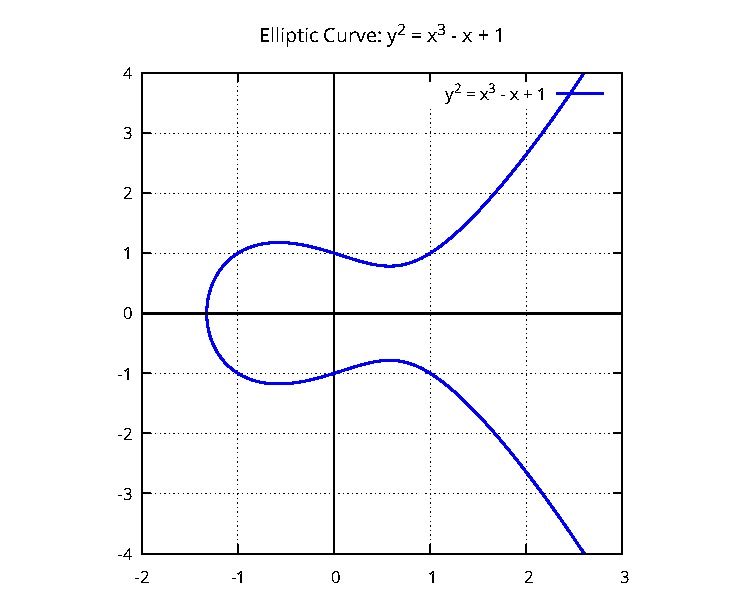
\includegraphics[width=0.5\textwidth]{elliptic_curve.pdf}
    \caption{楕円曲線の例}
  \end{figure}
\end{frame}

\begin{frame}{楕円曲線暗号のアルゴリズム}
  \begin{figure}
    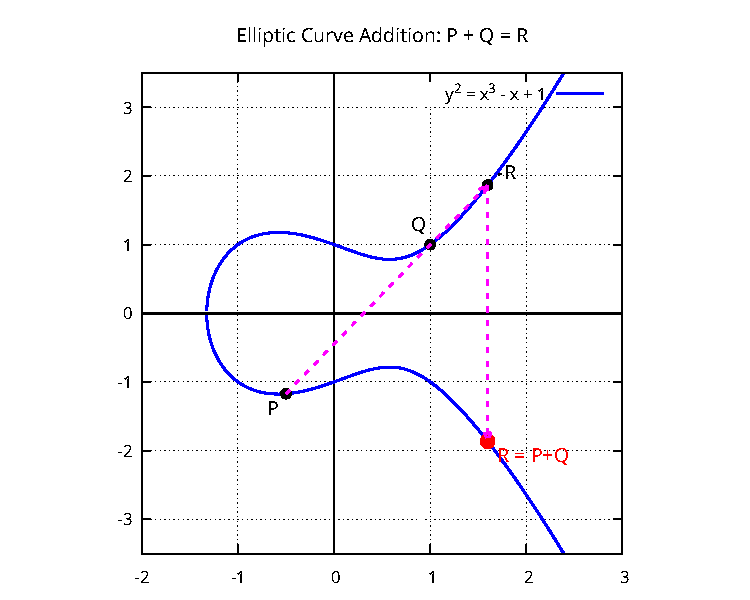
\includegraphics[width=0.5\textwidth]{ecc_addition.pdf}
    \caption{楕円曲線上の点の加算操作}
  \end{figure}
\end{frame}

\begin{frame}{楕円曲線暗号の秘密鍵と公開鍵}
  \begin{block}{秘密鍵と公開鍵の関係}
    楕円曲線暗号では，秘密鍵$d$は反射回数であり，公開鍵$P$は生成点$G$に秘密鍵$d$を掛けた点$P = dG$である．

    \vspace{1em}

    その他の要素は公開されている．
  \end{block}
\end{frame}

\end{document}
